\documentclass[11pt,a4paper]{article}

\usepackage[margin=1.8cm]{geometry}
\usepackage{booktabs}
\usepackage{graphicx}
\usepackage{hyperref}
\usepackage{enumitem}
\usepackage{array}

\hypersetup{
  colorlinks=true,
  linkcolor=black,
  urlcolor=blue,
  citecolor=black
}

\setlength{\parindent}{0em}
\setlength{\parskip}{0.45em}
\setlist[itemize]{leftmargin=1.8em,itemsep=0.1em,topsep=0.2em}

\title{\textbf{Embedding-Based Web Text Triage for Ancient Chinese Paleography}}
\author{}
\date{}

\begin{document}
\maketitle
\vspace{-1.4em}

\section{Research Question}

This project asks whether an embedding-based machine learning classifier can help triage short web text snippets for building a comprehensive corpus of Ancient Chinese paleography. Relevant web resources are spread across many types of sites. Some collect scholarly articles and philological discussions, some organize character forms and dictionary-style explanations, and others preserve images and transcriptions of oracle-bone, bronze-inscription, and excavated-manuscript materials. For corpus construction, the key question is therefore not only whether a snippet is related to paleography, but also what kind of material it is and how it should enter the corpus.

Manual filtering is possible at a small scale, but it quickly becomes impractical when the amount of web text grows. We therefore formulate the task as short-text classification: given a snippet from a public web source, the system predicts whether it is scholarly discussion, primary transcription, dictionary/reference content, or noise that should be discarded. The goal is not to replace expert interpretation, but to provide a practical first-pass routing tool for corpus building.

\section{Dataset and Labels}

Because large-scale web scraping can be ethically and technically ambiguous, this project uses 400 manually collected and annotated snippets instead of an automated crawler. Each row contains the text, label, source URL, and language. Sources include \textit{Lexicon of Pre-Qin Oracle, Bronze Inscriptions and Bamboo Scripts}, Xiaoxuetang, the Center for Research on Chinese Excavated Classics and Paleography at Fudan University, and the \textit{Multi-function Chinese Character Database}. The full source list is included in \texttt{source\_used.md}.

The final label set contains four classes, shown in Table \ref{tab:labels}. We also considered adding a separate metadata or catalogue-records class, such as object numbers, collection identifiers, bibliographic rows, database fields, and other structured records. We did not include it in the final scheme because this kind of information is highly structured rather than ordinary raw text. It is usually better handled by field extraction, table parsing, or source-specific database processing than by semantic short-text classification.

\begin{table}[h]
\centering
\small
\begin{tabular}{p{0.18\linewidth}p{0.74\linewidth}}
\toprule
\textbf{Label} & \textbf{Meaning} \\
\midrule
\texttt{kpt} & Primary transcription material, such as oracle-bone divinations, bronze inscriptions, excavated manuscript fragments, or other source-text transcriptions. \\
\texttt{kde} & Dictionary or reference entries, including character forms, meanings, pronunciations, glosses, variants, and cross-references. \\
\texttt{ksd} & Scholarly discussion, interpretive prose, research summaries, or paleographic argumentation. \\
\texttt{noise} & Navigation text, dates, login prompts, advertisements, unrelated text, broken OCR, or other material not suitable for the corpus. \\
\bottomrule
\end{tabular}
\caption{Final label set.}
\label{tab:labels}
\end{table}

The dataset is split into train, validation, and test sets with a 70/15/15 ratio: 280 training examples, 60 validation examples, and 60 test examples. Each class contains 100 examples in total and remains balanced across the splits.

\section{Method}

The project uses \texttt{intfloat/multilingual-e5-small} as the embedding model. This choice is practical for three reasons. First, the current data is mainly Chinese, but future paleography corpora may include English or Japanese scholarly discussion, so a multilingual model is more suitable than an English-only model. Second, the E5 family is designed for sentence embeddings and retrieval/classification settings, which fits the task of representing short snippets as semantic vectors. Third, \texttt{multilingual-e5-small} is lightweight enough for local experimentation and Hugging Face Space deployment.

We considered several alternatives. \texttt{BAAI/bge-small-en-v1.5} is a strong small embedding model, but it is mainly English-oriented and therefore less appropriate for a Chinese-centered dataset. \texttt{intfloat/e5-small-v2} is also lightweight, but it is not multilingual. \texttt{Qwen/Qwen3-Embedding-0.6B} may provide stronger Chinese representations, but it is larger and would make local training and Space deployment heavier. For this project, \texttt{multilingual-e5-small} offered the best balance between language coverage, performance, and deployment cost.

On top of the embeddings, we compared three classifiers: an average embedding baseline, logistic regression, and linear SVM. The average baseline assigns each example to the nearest class centroid. Logistic regression is a stable linear classifier for small datasets and provides class probabilities. Linear SVM is a strong standard baseline for high-dimensional text features. The final demo uses logistic regression because it tied with linear SVM on the test set while also supporting probability outputs for the Gradio interface. We considered a neural classifier such as a small MLP, but with only 400 examples, the risk of overfitting was high, and the traditional models already performed well.

\section{Evaluation}

The final logistic regression model achieved 0.9333 accuracy and 0.9298 macro F1 on the held-out test set, with 4 errors out of 60 examples. Table \ref{tab:perclass} gives the per-class precision, recall, and F1. The model performs very well on \texttt{kde}, \texttt{kpt}, and \texttt{noise}; all test errors come from \texttt{ksd}.

\begin{table}[h]
\centering
\small
\begin{tabular}{lrrrr}
\toprule
\textbf{Class} & \textbf{Precision} & \textbf{Recall} & \textbf{F1} & \textbf{Support} \\
\midrule
\texttt{kde} & 0.8824 & 1.0000 & 0.9375 & 15 \\
\texttt{kpt} & 0.9375 & 1.0000 & 0.9677 & 15 \\
\texttt{ksd} & 1.0000 & 0.7333 & 0.8462 & 15 \\
\texttt{noise} & 0.9375 & 1.0000 & 0.9677 & 15 \\
\midrule
\textbf{Macro avg} & 0.9393 & 0.9333 & 0.9298 & 60 \\
\bottomrule
\end{tabular}
\caption{Test-set classification report for logistic regression.}
\label{tab:perclass}
\end{table}

\begin{table}[h]
\centering
\small
\begin{tabular}{lrrrr}
\toprule
\textbf{Gold / Predicted} & \texttt{kde} & \texttt{kpt} & \texttt{ksd} & \texttt{noise} \\
\midrule
\texttt{kde} & 15 & 0 & 0 & 0 \\
\texttt{kpt} & 0 & 15 & 0 & 0 \\
\texttt{ksd} & 2 & 1 & 11 & 1 \\
\texttt{noise} & 0 & 0 & 0 & 15 \\
\bottomrule
\end{tabular}
\caption{Test-set confusion matrix for logistic regression.}
\label{tab:confusion}
\end{table}

\section{Error Analysis and Limitations}

All 4 test errors are \texttt{keep\_scholarly\_discussion} examples predicted as another class: 2 as \texttt{kde}, 1 as \texttt{kpt}, and 1 as \texttt{noise}. This suggests that \texttt{ksd} is the hardest label in the task. To inspect the embedding space, Figure \ref{fig:tsne} projects the E5 embeddings into two dimensions with t-SNE. Colors indicate gold labels, and black crosses mark the four logistic-regression test errors.

\begin{figure}[h]
\centering
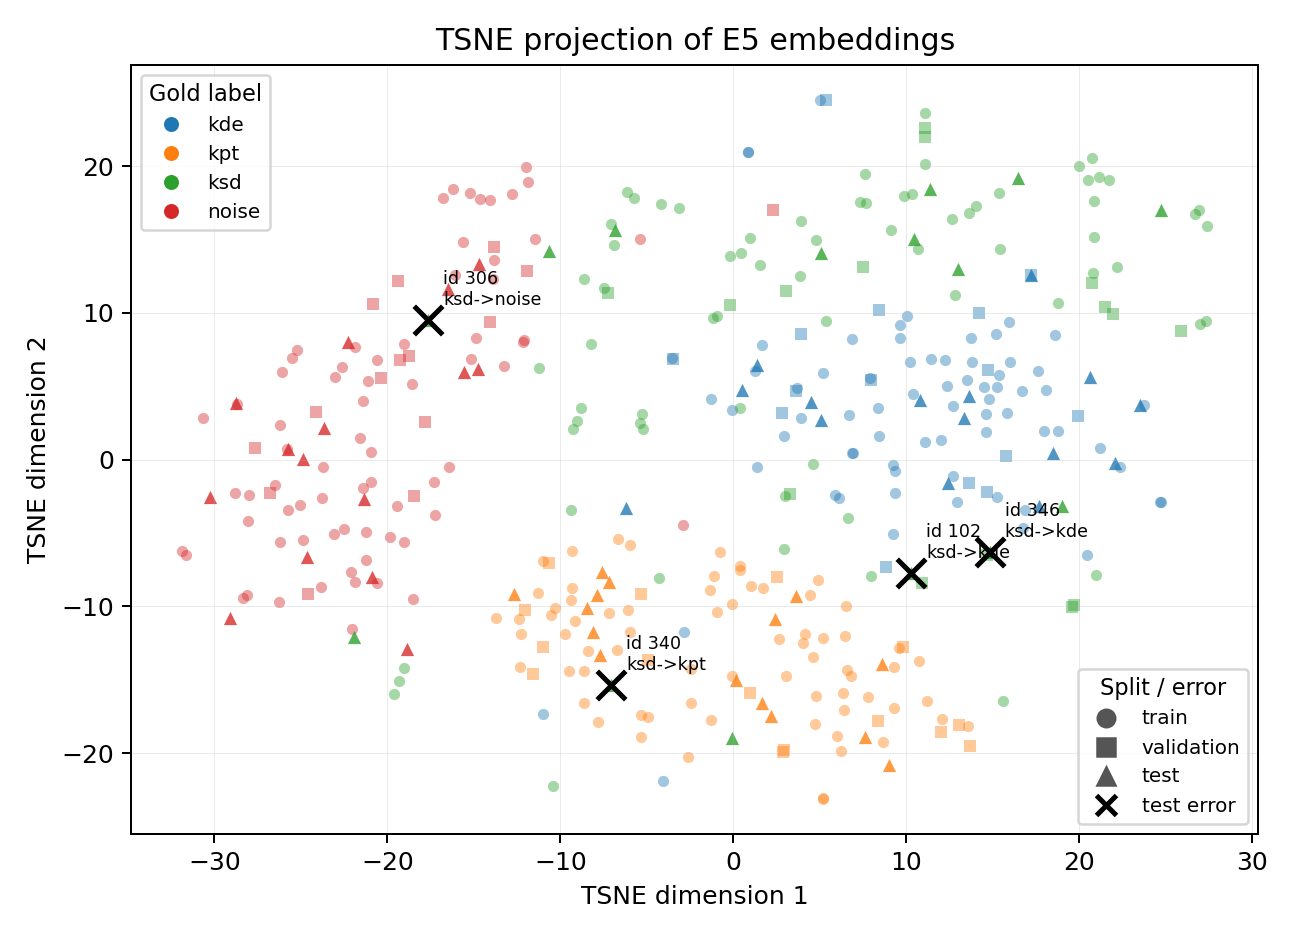
\includegraphics[width=0.82\linewidth]{figures/embedding_distribution_tsne.png}
\caption{t-SNE projection of E5 embeddings. Colors indicate gold labels, and black crosses mark the four logistic-regression test errors.}
\label{fig:tsne}
\end{figure}

The figure shows that \texttt{noise}, \texttt{kpt}, and \texttt{kde} form relatively visible regions, while \texttt{ksd} is more scattered and often lies between neighboring categories. This matches the confusion matrix: the model handles dictionary entries, primary transcriptions, and noise more consistently, but scholarly discussion can be absorbed by nearby classes. This is understandable in paleography. Scholarly prose often contains character explanations, phonological judgments, glosses, and dictionary-like conclusions. For example, a short sentence such as ``\textit{wan} and \textit{wan} have related initials and rhymes'' belongs to a scholarly argument in context, but its surface form resembles a dictionary note. Other scholarly passages directly quote primary material, making them close to \texttt{kpt}; short bibliographic or contextual notes may also resemble \texttt{noise}.

The project has several limitations. First, the dataset is mainly Chinese. Dictionary entries and primary transcriptions are almost entirely Chinese or Classical Chinese, while English and Japanese scholarly discussion are not systematically represented. As a result, the model may misclassify English or Japanese academic prose as \texttt{noise}. Second, the dataset is small, with only 400 examples, so the results may depend on source style and sampling choices. Third, the label boundaries are genuinely fuzzy: scholarly discussion, dictionary entries, and primary texts often appear together in paleographic writing. Finally, the model only uses isolated snippets and does not use page structure, titles, surrounding paragraphs, or source-site information; these signals could improve future versions.

\section{Deployment and AI Tool Reflection}

The project has been published as a Hugging Face Dataset, Model, and Space demo, with code, documentation, model files, results, and this report stored in the GitHub repository. AI coding assistance was used to design the pipeline, write training and evaluation scripts, inspect errors, build the Gradio demo, create embedding visualizations, and adjust the \LaTeX{} report. This greatly improved efficiency. Tasks such as scripting, demo development, plotting, and \LaTeX{} formatting could each have taken me one or two days to learn and debug independently. With Codex, I could complete them much faster through iterative prompting, which allowed me to focus more on theoretical analysis, annotation design, and experimental decisions.

AI also helped with report writing. Since English is not my first language, and my formal training in English academic writing started only last year, writing the report directly in English would have been slow. In this project, I first drafted the outline and analytical points in my native language, then used AI to insert experimental results, translate the report into an academic English style, and adjust the \LaTeX{} formatting. A task that might previously have taken a full day could be completed in about three hours. At the same time, this does not remove the need to keep improving my own writing; AI can also work as a feedback tool for learning academic English more quickly.

One surprising part of the process was that I could discuss the causes of model errors with AI, and its analysis was close to both my own interpretation and the pattern visible in the embedding visualization. For example, AI suggested that \texttt{ksd} could be confused with \texttt{kde}, \texttt{kpt}, and \texttt{noise}, which is exactly what the confusion matrix and t-SNE figure show. This was useful, but it also raised an ethical concern: when AI analysis sounds plausible, users may become less careful. It is therefore important to check claims against data, code, and visual evidence.

In this project, I did not observe serious AI hallucination, but I have seen it in other work. If users lack the relevant theoretical and technical background, they may be misled by fluent but incorrect AI output. Overall, AI can significantly improve research and development efficiency, but it also places high demands on the researcher's theoretical judgment, requires at least basic practical skills, and must be used with continuing attention to ethical issues such as data handling, interpretation, and responsibility.

\begin{itemize}
  \item Hugging Face Dataset: \url{https://huggingface.co/datasets/Harry214/paleography-web-text-triage-dataset}
  \item Hugging Face Model: \url{https://huggingface.co/Harry214/paleography-web-text-triage-logreg}
  \item Hugging Face Space: \url{https://huggingface.co/spaces/Harry214/paleography-web-text-triage-demo}
  \item GitHub repository: \url{https://github.com/hytung214-ai/paleography-web-text-triage}
\end{itemize}

\section*{References}

\begin{itemize}
  \item \textit{Lexicon of Pre-Qin Oracle, Bronze Inscriptions and Bamboo Scripts}.
  \item Xiaoxuetang.
  \item Center for Research on Chinese Excavated Classics and Paleography, Fudan University.
  \item \textit{Multi-function Chinese Character Database}.
  \item Full source list: \texttt{source\_used.md}.
\end{itemize}

\end{document}
